\begin{figure}[H]
  \centering
  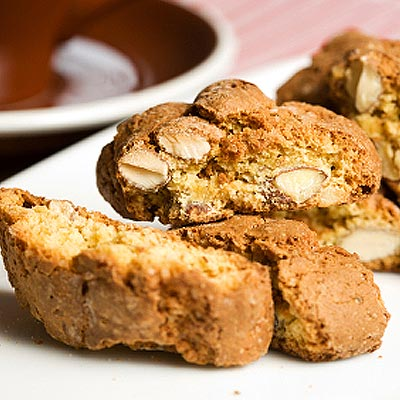
\includegraphics[width=0.65\textwidth]{cantuccini.JPG}
\end{figure}
\section{Cantuccini}
% Untertitel
\begin{centering}
% Wie viele werden satt?

\end{centering}
%\textbf{Zutaten:}
\begin{table}[H]
\centering
\begin{tabular*}{1\textwidth}{rlrl}
%& && \\
0.9\,oz / less then 2\,tbs.) & butter & 0.6\,oz / 1\,tbs & vanilla sugar \\
4.2\,oz / $\nicefrac{1}{2}$ cup & sugar & 6\,oz / 1 cup & peeled, coarsely chopped almonds \\
2 & eggs & & some drops bitter almond oil \\
8.8\,oz / 2 cups  & flour & & \\
\end{tabular*}
\end{table}
%Zubereitung:
\begin{Notes}
\item Preheat oven to 350°\,F.
\item Knead all ingredients together until well combined. Form 5 rolls.
\item Line a baking tray with baking paper and bake for 30-40\,min. While still hot cut into appox. 1\,cm thick slices. Bake for 10 more minutes.
\end{Notes}
\vfill
\newpage


\section*{Cantuccini}
% Untertitel
\begin{centering}
% Wie viele werden satt?

\end{centering}
%\textbf{Zutaten:}
\begin{table}[H]
\centering
\begin{tabular*}{1\textwidth}{rlrl}
%& && \\
25\,g & Butter &2 Pck. & Vanillezucker \\
120\,g & Zucker & 170\,g & geschälte, grob gehackte Mandeln \\
2 & Eier & & einige Tropfen Bittermandelöl \\
250\,g & Mehl & & \\
\end{tabular*}
\end{table}
%Zubereitung:
\begin{Notes}
\item Den Ofen auf 180°C vorheizen.
\item Alle Zutaten gut mit einander verkneten und 5 Rollen daraus formen.
\item Auf einem Backblech mit  Backpapier 30-40\,min backen. Noch heiß in ca. 1\,cm dicke Scheiben schneiden und weitere 10\,min backen.
\end{Notes}
\begin{figure}[H]
  \centering
  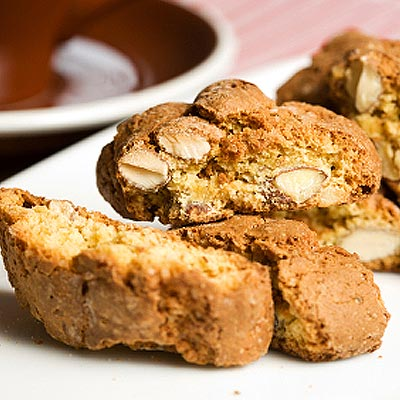
\includegraphics[width=0.65\textwidth]{cantuccini.JPG}
\end{figure}
\newpage

